%========================================
\section{Numerical Experiments} \label{sec:experiments}
To numerical validations, the proposed method is implemented in \texttt{Python3}
and tested on a laptop with an Intel Core i5-12500H CPU.
The solver~\texttt{GLOP}~\cite{glop} is adopted for linear and integer optimization.
Simulation videos can be found in the supplementary files.

%==============================
\subsection{System Description}\label{subsec:description}


%==============================
\begin{figure}[t]
    \centering
    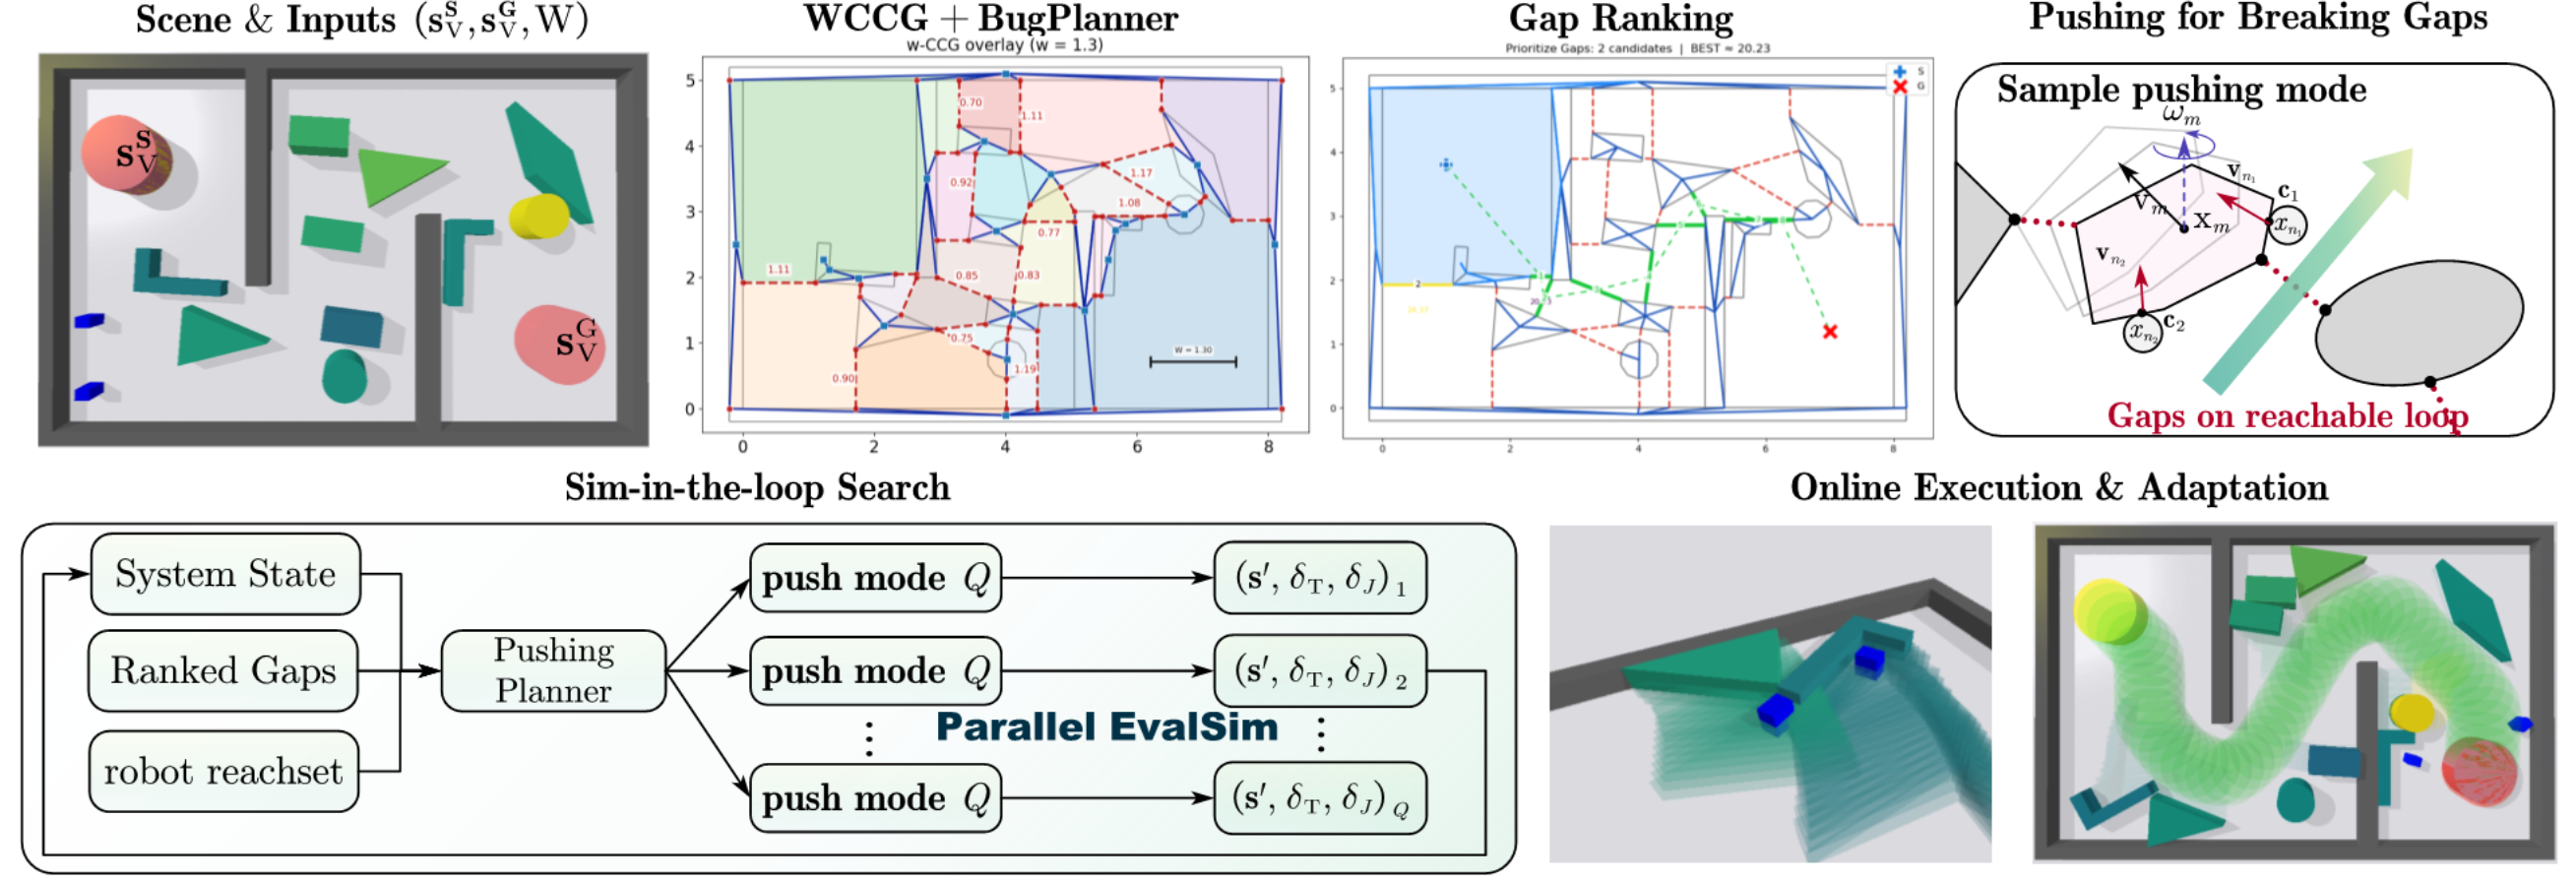
\includegraphics[width=0.97\hsize]{figures/overall.png}
    \vspace{-0.1in}
    \caption{\textbf{Top}: the number of subteams and their
      composition;
      \textbf{Bottom}: the status of agents in different modes
      and the number of tasks.
    }\label{fig:subteam}
    \vspace{-0.2in}
  \end{figure}
%==============================


%==============================
\subsection{Results}\label{subsec:results}
As shown in Fig.~\ref{fig:overall}


%==============================
\subsection{Comparisons}\label{subsec:comparisons}
The proposed method is compared against \textbf{{six}} baselines:


%====================
\begin{table}[t]
  \begin{center}
  \begin{threeparttable}
    \caption{Comparison with Baselines}\label{table:comparasion}
    \vspace{-0.05in}
    \setlength{\tabcolsep}{0.60\tabcolsep}
    \centering
    \renewcommand{\arraystretch}{1.1}
      \begin{tabular}{c c c |c| c c c c}
      \toprule
      \multicolumn{3}{c|}{Env.}& \multirow{2}{*}{\makecell{Methods}} & \multirow{2}{*}{\makecell{Resp. \\ Time[s]}} & \multirow{2}{*}{\makecell{Ave/Max \\ Plan Time[s]}} & \multirow{2}{*}{\makecell{T/W/X \\ Agents}} & \multirow{2}{*}{\makecell{Succ. \\ Rate[\%]}} \\
      \cline{1-3}
      N & M & J & & & & & \\
      \midrule
      \multirow{7}{*}{80} & \multirow{7}{*}{30} & \multirow{7}{*}{492} & \textbf{Ours} & {62.7} & {1.4/4.9} & {20/11/37} & {100} \\
      \multirow{7}{*}{} & \multirow{7}{*}{} & \multirow{7}{*}{} & \text{C-MILP-1} & {88.5} & {100/192} & {16/6/26} & {100} \\
      \multirow{7}{*}{} & \multirow{7}{*}{} & \multirow{7}{*}{} & \text{C-MILP-2} & {28.3} & {19/64} & {12/10/25} & {86} \\
      \multirow{7}{*}{} & \multirow{7}{*}{} & \multirow{7}{*}{} & \text{SAMP-1} & {108.3} & {54/92} & {19/8/24} & {100} \\
      \multirow{7}{*}{} & \multirow{7}{*}{} & \multirow{7}{*}{} & \text{SAMP-2} & {40.7} & {5.1/16} & {23/5/20} & {85} \\
      \multirow{7}{*}{} & \multirow{7}{*}{} & \multirow{7}{*}{} & \text{Inf-H} & {77.5} & {$> 15 \text{min}$} & {24/17/31} & {100} \\
      \multirow{7}{*}{} & \multirow{7}{*}{} & \multirow{7}{*}{} & \text{Greedy} & {112.1} & {0.3/0.6} & {33/9/30} & {100} \\
      \bottomrule
    \end{tabular}
  \end{threeparttable}
 \end{center}
  \vspace{-3mm}
  \end{table}
  % ====================

  %====================
 \begin{table}[t]
  \begin{center}
  \begin{threeparttable}
    \caption{SCALABILITY ANALYSIS}\label{table:scalability}
    \vspace{-0.05in}
    \setlength{\tabcolsep}{0.7\tabcolsep}
    \centering
    \renewcommand{\arraystretch}{1.1}
    \begin{tabular}{c c c c | c c c c}
      \toprule
      \multicolumn{4}{c|}{Env.} & \multirow{2}{*}{\makecell{Resp. \\ Time[s]}} & \multirow{2}{*}{\makecell{Ave/Max \\ Plan Time [s]}} & \multirow{2}{*}{\makecell{T/W/X \\ Agents}} & \multirow{2}{*}{\makecell{Succ. \\ Rate[\%]}}\\
      \cline{1-4}
      N & M & J & $\alpha$ & & & \\
      \midrule
      \multirow{2}{*}{120} & \multirow{2}{*}{50} & \multirow{2}{*}{824} & 0.05 & {95} & {1.6/4.6} & {33/10/39} & {100} \\
      \multirow{2}{*}{} & \multirow{2}{*}{} & \multirow{2}{*}{} & 0.1 & {102} & {1.7/4.9} & {26/9/35} & {100}\\
      \midrule
      \multirow{2}{*}{150} & \multirow{2}{*}{80} & \multirow{2}{*}{1319} & 0.05 & {153} & {1.8/5.1} & {37/12/37} & {100}\\
      \multirow{2}{*}{} & \multirow{2}{*}{} & \multirow{2}{*}{} & 0.1 & {165} & {2.1/6.2} & {12/11/34} & {97}\\
      \bottomrule
    \end{tabular}
  \end{threeparttable}
 \end{center}
  \vspace{-0.3in}
  \end{table}
  % ====================


 %==============================
  \subsection{Generalization}\label{subsec:scalability}
  For further validation, the fleet size is further increased
